\documentclass[crop,tikz]{standalone}
\usepackage[utf8]{inputenc}
\usepackage{tikz}
\usetikzlibrary{shapes.geometric, arrows}

\tikzstyle{startstop} = [rectangle, rounded corners, minimum width=2cm, minimum height=1cm, text centered, draw=black, fill=red!30]
\tikzstyle{io} = [trapezium, trapezium left angle=70, trapezium right angle=110, minimum width=2cm, minimum height=1cm, text centered, draw=black, fill=blue!30]
\tikzstyle{process} = [rectangle, minimum width=2cm, minimum height=1cm, text centered, draw=black, fill=orange!30]
\tikzstyle{decision} = [diamond, minimum width=2cm, minimum height=1cm, text centered, draw=black, fill=green!30]
\tikzstyle{arrow} = [thick, ->, >=stealth]

\begin{document}
	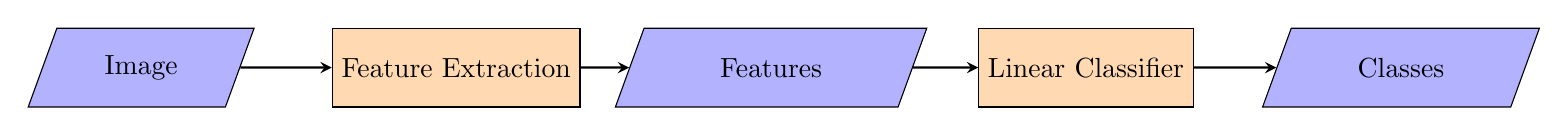
\begin{tikzpicture}[node distance=4cm]
	\node (in1) [io] {Image};
	\node (fe) [process, right of=in1] {Feature Extraction};
	\node (feat) [io, right of=fe] {Features};
	\node (lc) [process, right of=feat] {Linear Classifier};
	\node (cl) [io, right of=lc] {Classes};
	
	\draw [arrow] (in1) -- (fe);
	\draw [arrow] (fe) -- (feat);
	\draw [arrow] (feat) -- (lc);	
	\draw [arrow] (lc) -- (cl);
	\end{tikzpicture}
\end{document}